% The compressed quadrature-point store: the pulled-back tangent at each point, encoded, in the
% blocked layout (a block of V elements, numbers ordered point, component, lane).
\documentclass[border=2pt]{standalone}
% Shared preamble of the format diagrams: colours of the paper's figures (paper_figures.py) and
% the drawing styles.  Each diagram is a standalone document built to a PDF of the text width.
\usepackage{amsmath,amssymb}
\usepackage{tikz}
\usetikzlibrary{arrows.meta,calc,decorations.pathreplacing,patterns,positioning}

\definecolor{cindex}{HTML}{BDBDBD}  % column indices, offsets, row pointers
\definecolor{cvalue}{HTML}{6E6E6E}  % floating-point values (BSR)
\definecolor{cpoint}{HTML}{1B9E77}  % quadrature-point store
\definecolor{celem}{HTML}{1F78B4}   % element matrix
\definecolor{cqbsr}{HTML}{A6761D}   % quantized BSR
\definecolor{cscale}{HTML}{E6AB02}  % scales
\definecolor{cmean}{HTML}{7570B3}   % f32 element mean

\tikzset{
  >={Stealth[length=4pt]},
  grid/.style={draw=black!45, line width=0.25pt},
  frame/.style={draw=black!70, line width=0.5pt},
  title/.style={font=\small\bfseries, anchor=west, inner sep=0pt},
  lab/.style={font=\footnotesize, inner sep=1pt},
  note/.style={font=\scriptsize, text=black!75, inner sep=1pt, execute at begin node={\hyphenpenalty=10000\exhyphenpenalty=10000}},
  num/.style={font=\tiny, inner sep=0pt},
  brace/.style={decorate, decoration={brace, amplitude=3pt, raise=1pt}, line width=0.4pt},
  arr/.style={->, line width=0.5pt, black!70},
  pad/.style={pattern=north east lines, pattern color=black!30},
}

% \cell{x}{y}{w}{h}{fill}: a filled rectangle with a thin outline, lower-left corner at (x,y).
\newcommand{\cell}[5]{\filldraw[fill=#5, grid] (#1,#2) rectangle ++(#3,#4);}
% \blk{x}{y}{s}{fill}: a 3x3 block of side s with its 3x3 entry grid.
\newcommand{\blk}[4]{%
  \filldraw[fill=#4, grid] (#1,#2) rectangle ++(#3,#3);
  \draw[draw=white, line width=0.25pt] (#1,#2) ++(#3/3,0) -- ++(0,#3) ++(#3/3,0) -- ++(0,-#3);
  \draw[draw=white, line width=0.25pt] (#1,#2) ++(0,#3/3) -- ++(#3,0) ++(0,#3/3) -- ++(-#3,0);
  \draw[grid] (#1,#2) rectangle ++(#3,#3);}
% \vthree{x}{y}{fill}: a 3-vector (one node's components) as three small cells, left end at (x,y).
\newcommand{\vthree}[3]{\foreach \k in {0,1,2} \filldraw[fill=#3, grid] (#1+\k*0.14,#2) rectangle ++(0.14,0.14);}
% \op{x}{y}{symbol}: an operation in a small circle.
\newcommand{\op}[3]{\node[circle, draw=black!70, line width=0.4pt, inner sep=0.5pt, minimum size=9pt, font=\tiny] at (#1,#2) {#3};}

\begin{document}
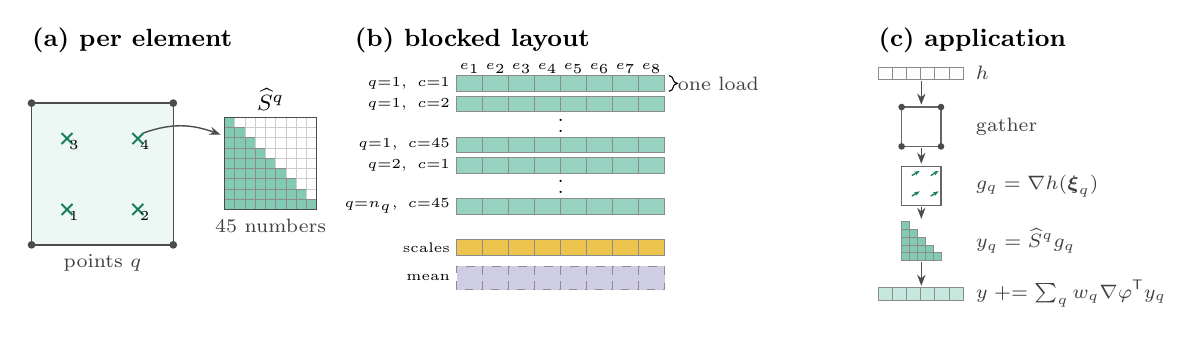
\begin{tikzpicture}
  % ---------------------------------------------------------------- (a) what is stored
  \node[title] at (0, 3.35) {(a) per element};
  \filldraw[fill=cpoint!8, draw=black!70, line width=0.5pt] (0,0.75) rectangle (1.8,2.55);
  \foreach \x/\y [count=\q] in {0.45/1.2, 1.35/1.2, 0.45/2.1, 1.35/2.1} {
    \draw[cpoint!80!black, line width=0.7pt] (\x-0.07,\y-0.07) -- (\x+0.07,\y+0.07) (\x-0.07,\y+0.07) -- (\x+0.07,\y-0.07);
    \node[num, anchor=north west] at (\x+0.02,\y-0.02) {$\q$};
  }
  \foreach \x/\y in {0/0.75, 1.8/0.75, 0/2.55, 1.8/2.55} \fill[black!70] (\x,\y) circle (1.4pt);
  \node[note, anchor=north] at (0.9, 0.67) {points $q$};
  \def\t{0.13}
  \begin{scope}[shift={(2.45,1.2)}]
    \foreach \r in {0,...,8} \foreach \c in {0,...,8} {
      \pgfmathparse{\c<=\r ? 1 : 0}
      \ifnum\pgfmathresult=1
        \filldraw[fill=cpoint!55, grid] (\c*\t, {(8-\r)*\t}) rectangle ++(\t,\t);
      \else
        \draw[grid, draw=black!20] (\c*\t, {(8-\r)*\t}) rectangle ++(\t,\t);
      \fi
    }
    \draw[frame] (0,0) rectangle (9*\t, 9*\t);
    \node[lab, anchor=south] at (4.5*\t, 9*\t+0.05) {$\widehat S^{q}$};
    \node[note, anchor=north] at (4.5*\t, -0.08) {$45$ numbers};
  \end{scope}
  \draw[arr] (1.42,2.17) to[out=20, in=160] (2.4,2.15);

  % ---------------------------------------------------------------- (b) the blocked layout
  \begin{scope}[shift={(5.4,0)}]
    \def\w{0.33}\def\h{0.2}
    \node[title] at (-1.3, 3.35) {(b) blocked layout};
    \foreach \v in {1,...,8} \node[num, anchor=south] at ({(\v-0.5)*\w}, 2.92) {$e_{\v}$};
    \foreach \lbl [count=\k from 0] in {{$q{=}1,\ c{=}1$}, {$q{=}1,\ c{=}2$}, {}, {$q{=}1,\ c{=}45$}, {$q{=}2,\ c{=}1$}, {}, {$q{=}n_q,\ c{=}45$}} {
      \pgfmathsetmacro{\y}{2.7-\k*(\h+0.06)}
      \ifx\lbl\empty
        \node[font=\scriptsize, inner sep=0pt] at (4*\w, \y+\h/2+0.02) {$\vdots$};
      \else
        \foreach \v in {0,...,7} {\cell{\v*\w}{\y}{\w}{\h}{cpoint!45}}
        \node[num, anchor=east] at (-0.08, \y+\h/2) {\lbl};
      \fi
    }
    \foreach \v in {0,...,7} {\cell{\v*\w}{0.62}{\w}{\h}{cscale!70}}
    \node[num, anchor=east] at (-0.08, 0.72) {scales};
    \foreach \v in {0,...,7} {\filldraw[fill=cmean!35, grid, dashed] (\v*\w, 0.18) rectangle ++(\w, 0.3);}
    \node[num, anchor=east] at (-0.08, 0.33) {mean};
    \draw[brace] (8*\w+0.02, 2.7+\h) -- (8*\w+0.02, 2.7) node[midway, right=3pt, note] {one load};
  \end{scope}

  % ---------------------------------------------------------------- (c) the application, one lane
  \begin{scope}[shift={(10.75,0)}]
    \node[title] at (0, 3.35) {(c) application};
    \def\xc{0.55}
    % global h
    \foreach \k in {0,...,5} {\cell{\k*0.18}{2.85}{0.18}{0.16}{white}}
    \node[note, anchor=west] at (1.2, 2.93) {$h$};
    % element nodes
    \draw[black!60, line width=0.4pt] (\xc-0.25,2.0) rectangle (\xc+0.25,2.5);
    \foreach \x/\y in {-0.25/2.0, 0.25/2.0, -0.25/2.5, 0.25/2.5} \fill[black!70] (\xc+\x,\y) circle (1.2pt);
    \node[note, anchor=west] at (1.2, 2.25) {gather};
    % gradients at the points
    \draw[black!60, line width=0.4pt] (\xc-0.25,1.25) rectangle (\xc+0.25,1.75);
    \foreach \x/\y in {-0.12/1.37, 0.12/1.37, -0.12/1.63, 0.12/1.63}
      \draw[cpoint!80!black, line width=0.5pt, ->, >={Stealth[length=2pt]}] (\xc+\x,\y) -- ++(0.1,0.06);
    \node[note, anchor=west] at (1.2, 1.5) {$g_q = \nabla h(\boldsymbol{\xi}_q)$};
    % the stored tangent
    \foreach \r in {0,...,4} \foreach \c in {0,...,4} {
      \pgfmathparse{\c<=\r ? 1 : 0}
      \ifnum\pgfmathresult=1 \filldraw[fill=cpoint!55, grid] (\xc-0.25+\c*0.1, {1.05-\r*0.1}) rectangle ++(0.1,-0.1); \fi
    }
    \node[note, anchor=west] at (1.2, 0.8) {$y_q = \widehat S^{q} g_q$};
    % element output, scattered
    \foreach \k in {0,...,5} {\cell{\k*0.18}{0.05}{0.18}{0.16}{cpoint!25}}
    \node[note, anchor=west] at (1.2, 0.13) {$y \mathrel{+}= \sum_q w_q \nabla\varphi^{\mathsf T} y_q$};
    \foreach \a/\b in {2.83/2.53, 1.98/1.78, 1.23/1.08, 0.53/0.23} \draw[arr] (\xc,\a) -- (\xc,\b);
  \end{scope}
\end{tikzpicture}
\end{document}
